\begin{usecase}{Manage Scheduling Conflicts}
  \ucbasicinfo{Medium}{Regular}
  \ucshortdescription{This UC allows users to view and manage all unresolved scheduling conflicts in their calendar through a dedicated interface.}
  \uctrigger{This UC is triggered when the user opens the Conflicts view in the iOS app.}
  \ucactors{User}{iOS App}
  \ucpreconditions{
    \begin{itemize}
      \item The iOS app is installed and running
      \item Calendar access is authorized
      \item There are unresolved conflicts in the ConflictManager
    \end{itemize}
  }
  \ucrelationships{N/A}{N/A}{N/A}
  \ucinputsoutputs{
    \begin{itemize}
      \item \textbf{Unresolved conflicts} (Source: ConflictManager)
      \item \textbf{User resolution choices} (Source: User Interface)
    \end{itemize}
  }{
    \begin{itemize}
      \item \textbf{Updated calendar events} (Destination: iOS Calendar)
      \item \textbf{Updated conflict status} (Destination: ConflictManager)
    \end{itemize}
  }
  \ucmainflow{
    \begin{enumerate}
      \item The user opens the Conflicts view in the app
            \ucinfo{The app displays a list of all unresolved conflicts using ConflictRowView for each conflict.}
      \item For each conflict, the user can:
            \ucinfo{
              \begin{itemize}
                \item View the conflicting events in a timeline visualization
                \item See the event titles, times, and number of conflicts
                \item Select a conflict to resolve
              \end{itemize}
            }
      \item When selecting a conflict, the user is presented with resolution options
            \ucinfo{The ConflictResolutionView presents three options:
              \begin{itemize}
                \item Keep All Events - Leave events as is with known conflict
                \item Reschedule Event - Move the new event to a different time
                \item Cancel Event - Remove the new event from the calendar
              \end{itemize}
            }
      \item The user can visualize the impact of their choice
            \ucinfo{The ConflictTimelineView provides a visual representation of:
              \begin{itemize}
                \item Current event positions
                \item Proposed new time (when rescheduling)
                \item Conflict resolution preview
              \end{itemize}
            }
    \end{enumerate}
  }
  \ucalternateflows{
    \begin{enumerate}
      \item If no unresolved conflicts exist:
            \ucinfo{The app displays a "No Scheduling Conflicts" message with a checkmark.}
      \item If the user dismisses without resolving:
            \ucinfo{The conflict remains in the unresolved state and can be addressed later.}
    \end{enumerate}
  }
  \ucexceptions{
    \begin{itemize}
      \item If calendar access is revoked, the app prompts for re-authorization
      \item If event modification fails, the conflict remains unresolved and can be retried
    \end{itemize}
  }
  \ucconclusion{The UC ends when the user has reviewed and optionally resolved their calendar conflicts.}
  \ucpostconditions{
    \begin{itemize}
      \item Resolved conflicts are marked as such in the ConflictManager
      \item Calendar events reflect any changes made through conflict resolution
      \item Remaining unresolved conflicts are preserved for later
    \end{itemize}
  }
  \ucspecialrequirements{
    \begin{itemize}
      \item The interface must provide clear visual feedback through the timeline view
      \item Resolution options must be easily accessible and understandable
      \item The system must maintain conflict state across app sessions
    \end{itemize}
  }
\end{usecase}

\begin{figure}[!h]
  \centering
  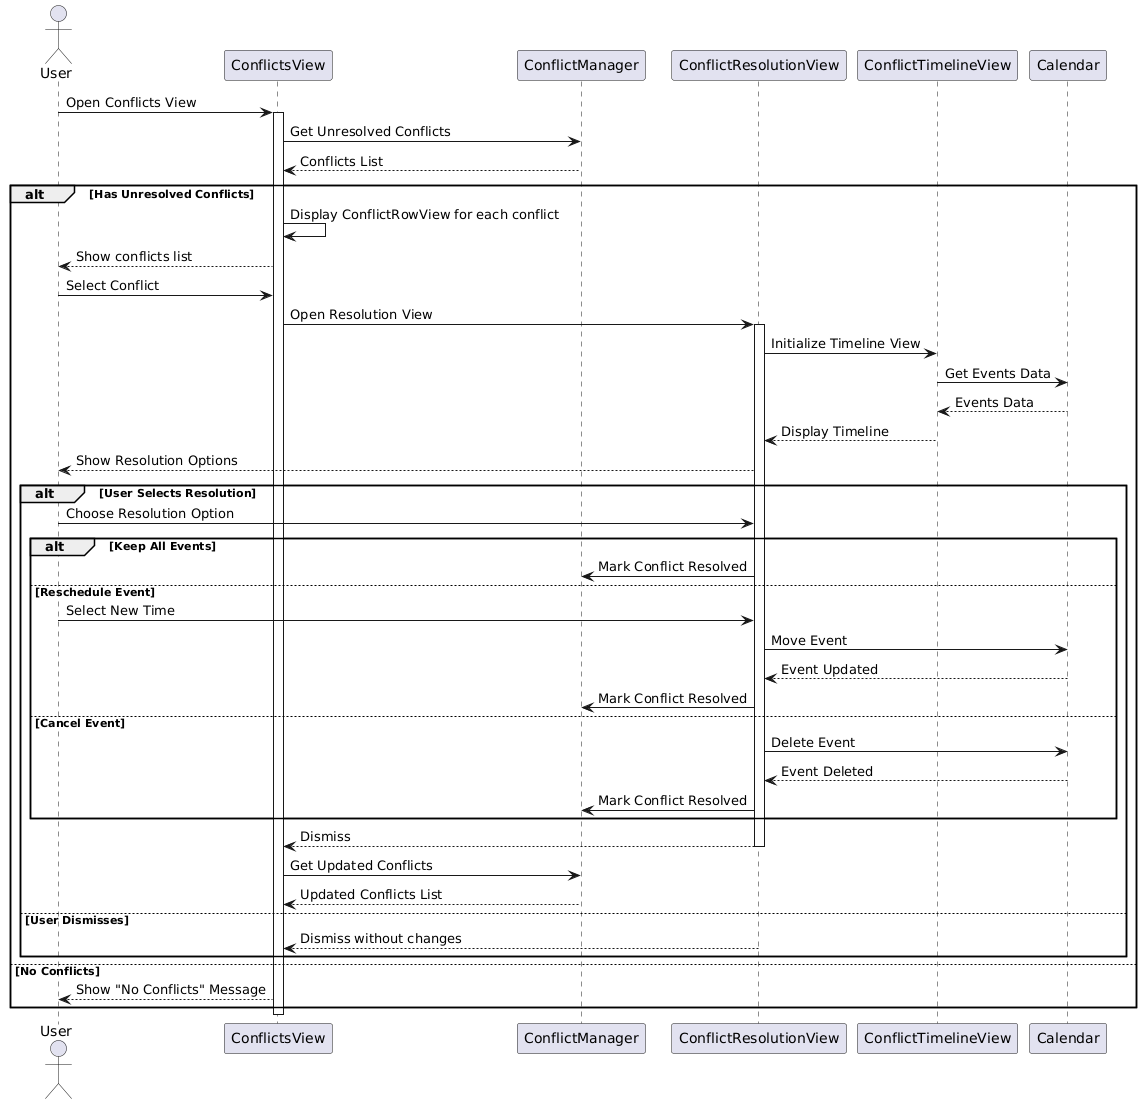
\includegraphics[width=\textwidth]{images/docs/diagrams/sequence-diagrams/all-sequence-diagrams/Manage Scheduling Conflicts.png}
  \caption{Manage Scheduling Conflicts Sequence Diagram}
  \label{fig:seq/manage-scheduling-conflicts}
\end{figure}

The sequence diagram in Figure~\ref{fig:seq/manage-scheduling-conflicts} illustrates how users can manage their calendar conflicts through the iOS app's dedicated Conflicts view. This interface serves as a central hub for reviewing and resolving all scheduling conflicts.

The process leverages several key components:
\begin{itemize}
  \item \textbf{ConflictManager}: Maintains the state of all conflicts and their resolution status
  \item \textbf{ConflictsView}: Provides the main interface listing all unresolved conflicts
  \item \textbf{ConflictResolutionView}: Offers the resolution interface with timeline visualization
  \item \textbf{ConflictTimelineView}: Delivers an interactive visual representation of conflicts
\end{itemize}

This implementation ensures that users can:
\begin{itemize}
  \item View all their conflicts in one place
  \item Understand conflicts through visual timeline representation
  \item Make informed decisions about resolution
  \item Address conflicts at their convenience
\end{itemize}

The system maintains conflicts until they are explicitly resolved, allowing users to manage their schedule conflicts efficiently while ensuring no scheduling issues go unnoticed.